\documentclass[11pt]{article}

\usepackage[utf8]{inputenc} % Required for inputting international characters
\usepackage[T1]{fontenc} % Output font encoding for international characters
\usepackage{listings}
\usepackage{xcolor}
\usepackage{graphicx}
\usepackage{multirow}

	\addtolength{\oddsidemargin}{-.875in}
	\addtolength{\evensidemargin}{-.875in}
	\addtolength{\textwidth}{1.75in}

	\addtolength{\topmargin}{-.875in}
	\addtolength{\textheight}{1.75in}
	
	\lstset
	{ %Formatting for code in appendix
	keywordstyle=\color{blue},
	commentstyle = \color{gray},
    language=Verilog,
    basicstyle=\footnotesize,
    numbers=left,
    stepnumber=1,
    showstringspaces=false,
    tabsize=1,
    breaklines=true,
    breakatwhitespace=false,
	}
	
\makeatletter
\newcommand*{\Xbar}{}%
\DeclareRobustCommand*{\Xbar}{%
  \mathpalette\@Xbar{}%
}
\newcommand*{\@Xbar}[2]{%
  % #1: math style
  % #2: unused (empty)
  \sbox0{$#1\mathrm{X}\m@th$}%
  \sbox2{$#1X\m@th$}%
  \rlap{%
    \hbox to\wd2{%
      \hfill
      $\overline{%
        \vrule width 0pt height\ht0 %
        \kern\wd0 %
      }$%
    }%
  }%
  \copy2 %
}
\makeatother
\begin{document}

\begin{titlepage} 

	\newcommand{\HRule}{\rule{\linewidth}{0.5mm}} 
	
	\center 
	
	\textsc{\huge National Institute of Technology}\\[0.5cm] 
	\textsc{\LARGE DURGAPUR}\\[2.5cm]
	
	\textsc{\Large Design and Analysis of Algorithms }\\[0.5cm] 
	
	\textsc{\large CSS-551}\\[1.5cm] % Minor heading such as course title
	
	\HRule\\[0.4cm]
	
	{\huge\bfseries Lab Report }\\[0.1cm] % Title of your document
	
	\HRule\\[1.5cm]

	
	{\LARGE \textsc{Prasun Kumar Bhuin}}\\[0.3cm] % Your name
    {\large 18CS8028}\\[0.3cm]
	
	\vfill\vfill\vfill % Position the date 3/4 down the remaining page
	
	{\large 30 April, 2021} % Date, change the \today to a set date if you want to be precise

	%\vfill % Push the date up 1/4 of the remaining page
	
\end{titlepage}
\tableofcontents

\newpage


\section{Exponential vs Polynomial Running time solution Fibonacci Sequence}
	\subsection{Code}
		\lstinputlisting[language=C++, frame = single]{code/1.cpp}
	\subsection{Output}
		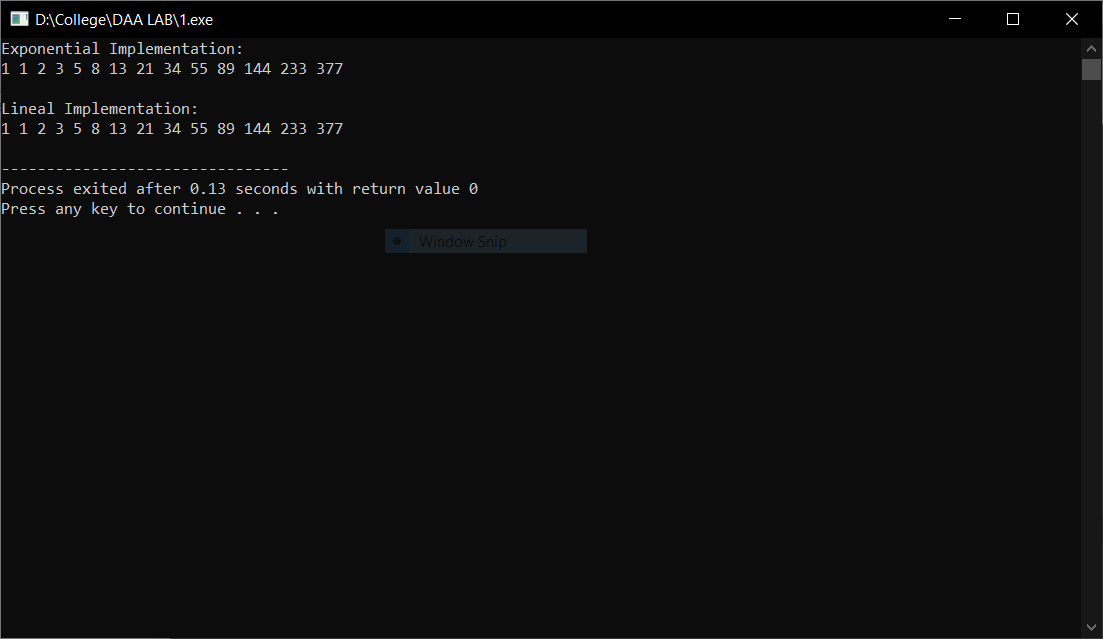
\includegraphics[scale=0.7]{pic/1.png}
\newpage









\section{Heap and Priority Queue}
	\subsection{Code}
		\lstinputlisting[language=C++, frame = single]{code/2.cpp}
	\subsection{Output}
		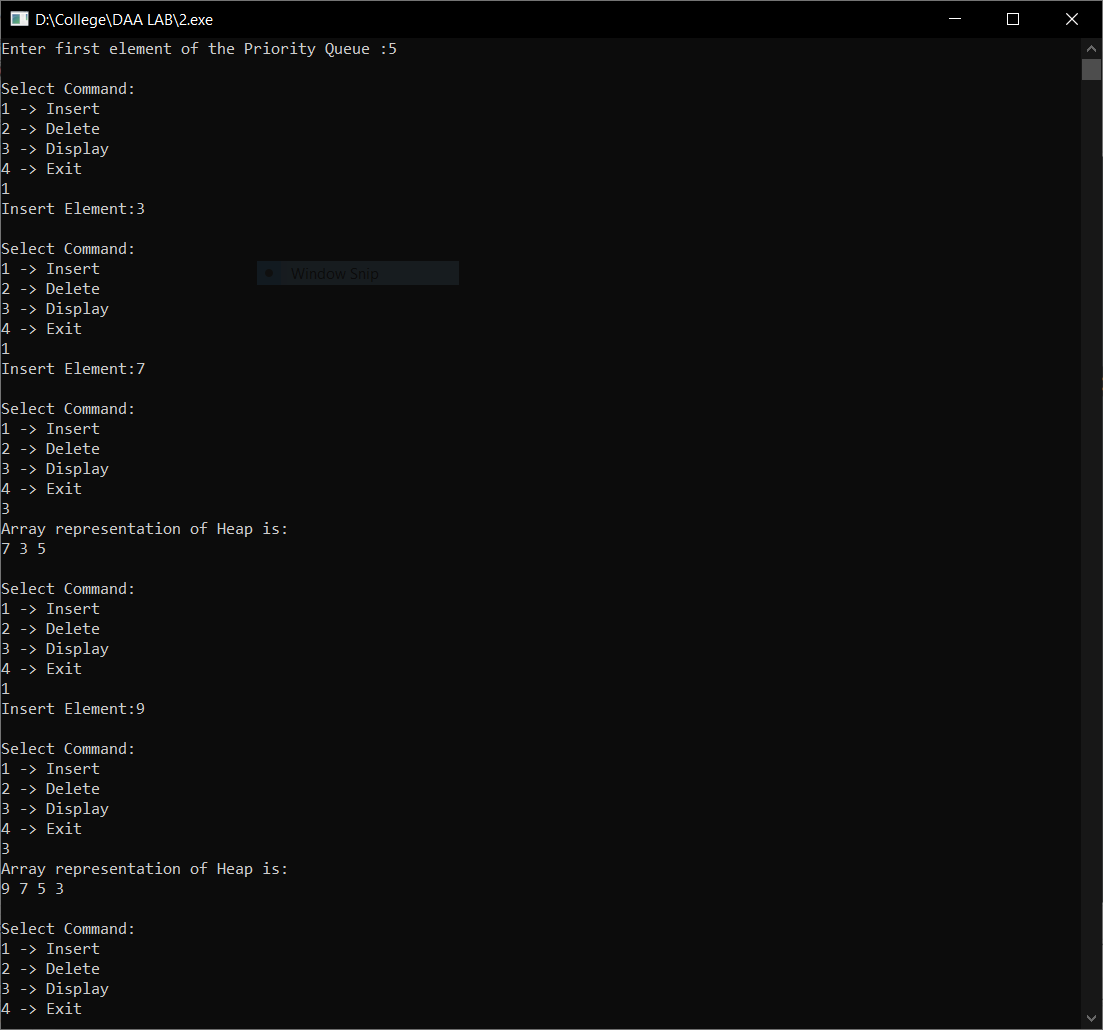
\includegraphics[scale=0.7]{pic/2.png}
\newpage










\section{Counting Sort}
	\subsection{Code}
		\lstinputlisting[language=C++, frame = single]{code/3.cpp}
	\subsection{Output}
		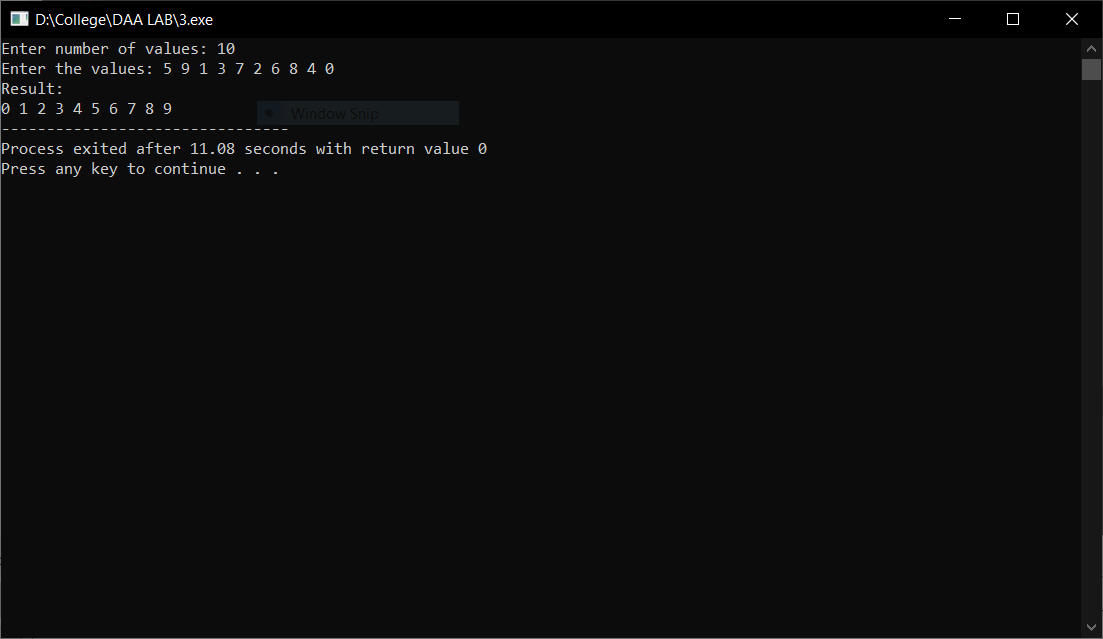
\includegraphics[scale=0.7]{pic/3.png}
\newpage











\section{Merge Sort}
	\subsection{Code}
		\lstinputlisting[language=C++, frame = single]{code/4.cpp}
	\subsection{Output}
		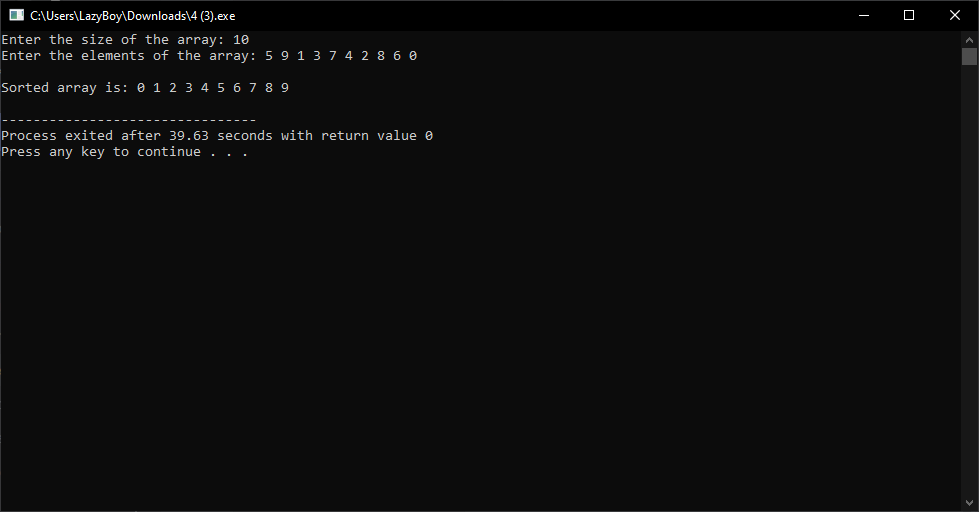
\includegraphics[scale=0.7]{pic/4.png}
\newpage










\section{Fractional Knapsack Problem}
	\subsection{Code}
		\lstinputlisting[language=C++, frame = single]{code/5.cpp}
	\subsection{Output}
		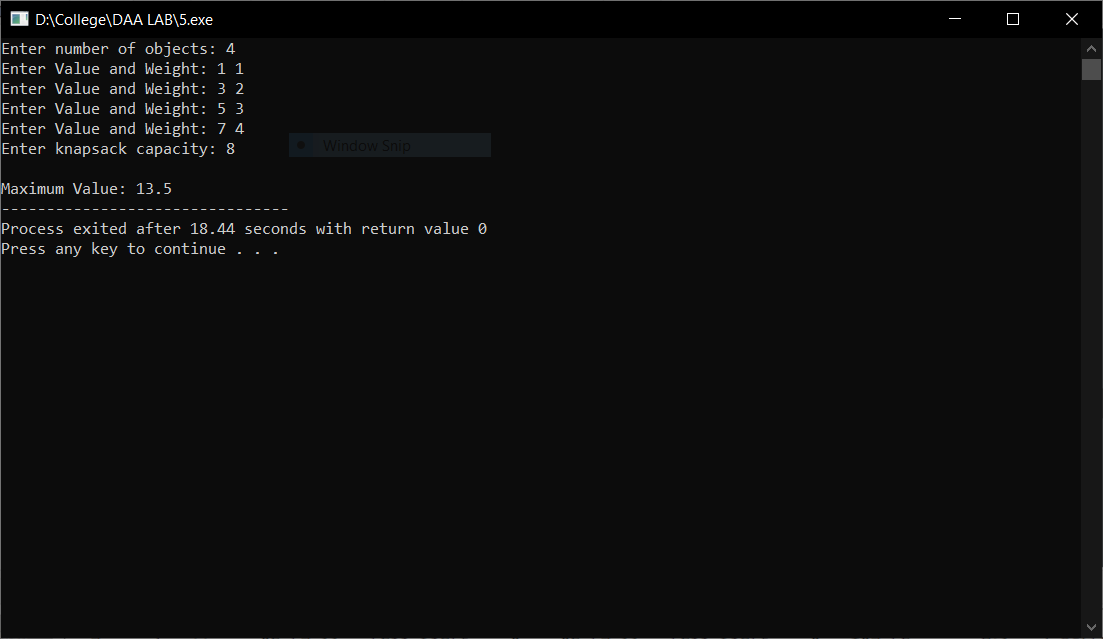
\includegraphics[scale=0.7]{pic/5.png}
\newpage








\section{Longest Common Subsequence Algorithm}
	\subsection{Question}
	\subsection{Code}
		\lstinputlisting[language=C++, frame = single]{code/6.cpp}
	\subsection{Output}
		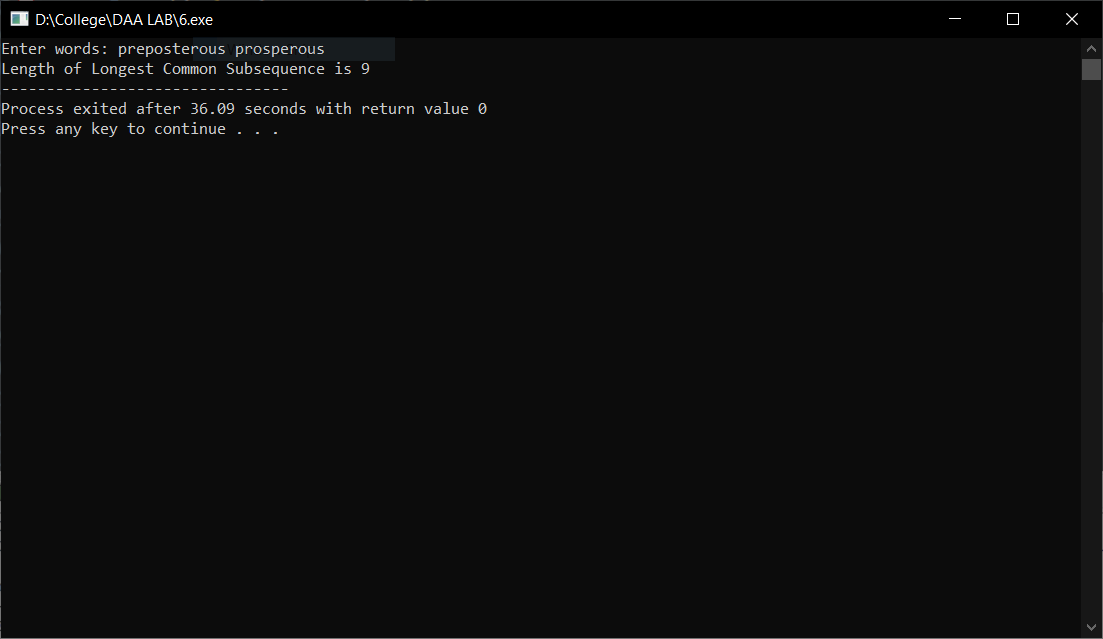
\includegraphics[scale=0.7]{pic/6.png}
\newpage









\section{Depth First Search in a Graph}
	\subsection{Question}
	\subsection{Code}
		\lstinputlisting[language=C++, frame = single]{code/7.cpp}
	\subsection{Output}
		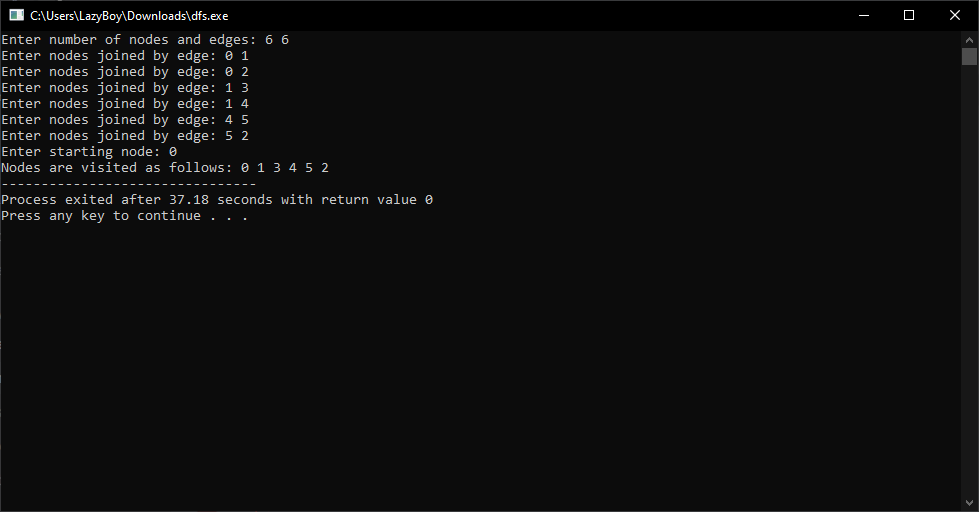
\includegraphics[scale=0.7]{pic/7.png}
\newpage









\section{Finding Kth smallest element in worst case linear time}
	\subsection{Code}
		\lstinputlisting[language=C++, frame = single]{code/8.cpp}
	\subsection{Output}
		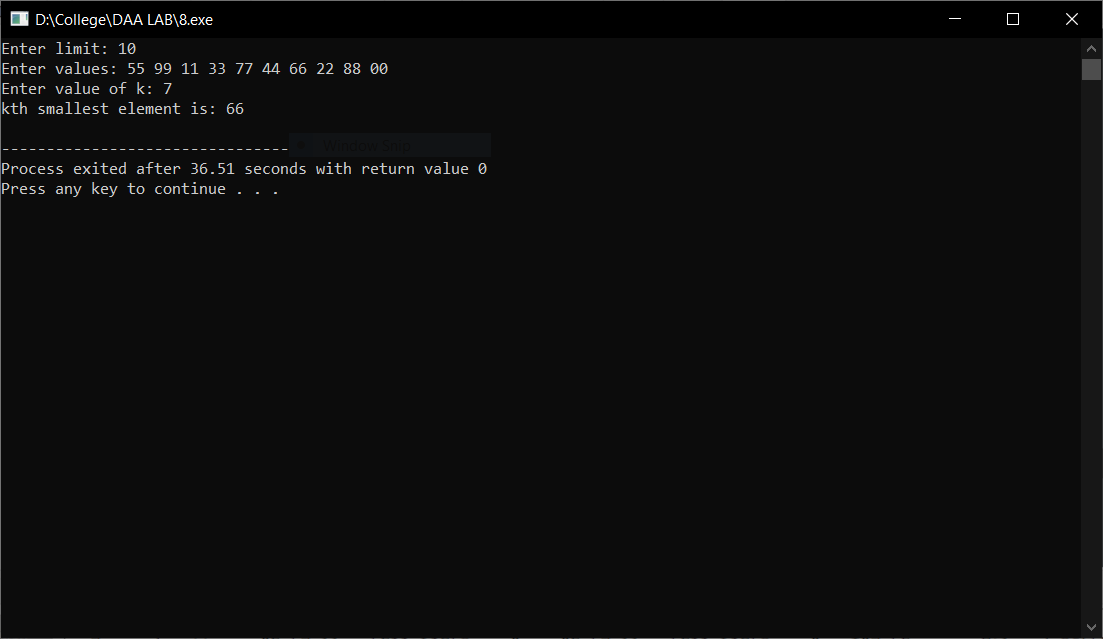
\includegraphics[scale=0.7]{pic/8.png}
\newpage








\section{Randomised Quick Sort}
	\subsection{Code}
		\lstinputlisting[language=C++, frame = single]{code/9.cpp}
	\subsection{Output}
		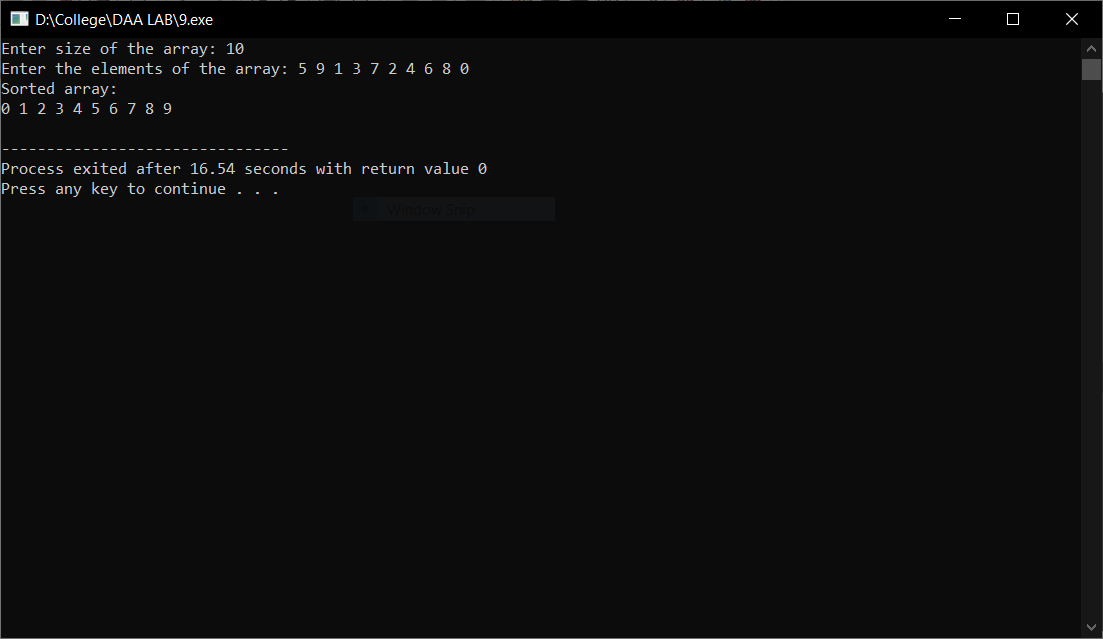
\includegraphics[scale=0.7]{pic/9.png}
\newpage









\section{Convex Hull computation in 2D}
	\subsection{Code}
		\lstinputlisting[language=C++, frame = single]{code/10.cpp}
	\subsection{Output}
		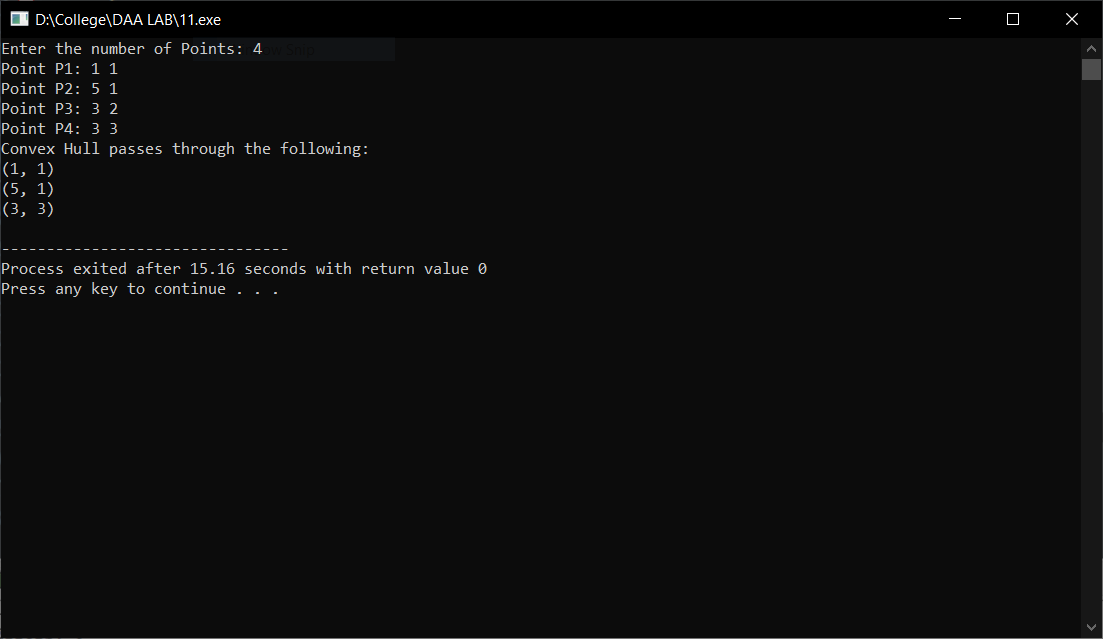
\includegraphics[scale=0.7]{pic/10.png}
\newpage








\end{document}
